\section{NSGA-II Matrix}

The NSGA-II matrix captures key performance metrics of the algorithm over successive generations, including the average, standard deviation, minimum, and maximum objective values. These indicators provide valuable insights into the optimization dynamics, enabling the assessment of both convergence behavior and population diversity. The average reflects the overall improvement in solution quality, while the standard deviation indicates the spread and diversity within the population. Minimum and maximum values represent the boundaries of the explored solution space in each generation. Such matrix-based analysis is essential for understanding how NSGA-II balances exploration and exploitation in multi-objective optimization \cite{A Fast and Elitist Multi-objective Genetic Algorithm: NSGA-II}. Figure~\ref{fig:nsga2_metrics} illustrates these performance trends across generations, helping to visualize the algorithm’s effectiveness over time.

\begin{figure}[h!]
    \centering
    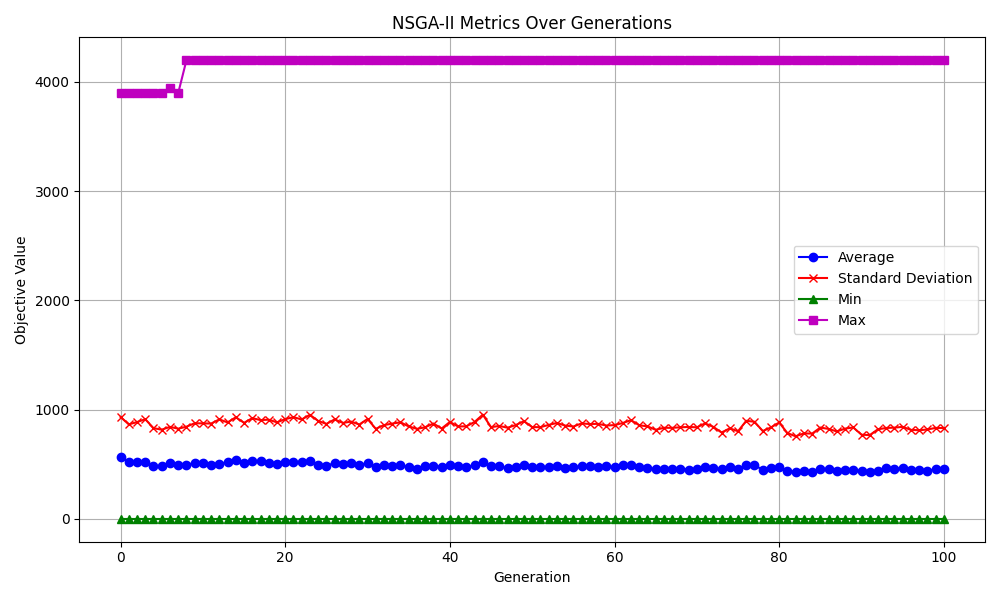
\includegraphics[width=0.8\textwidth]{../Figures/nsga2_metrics.png}
    \caption{Performance metrics of NSGA-II over generations}
    \label{fig:nsga2_metrics}
\end{figure}
\newpage
However, the NSGA-II matrix shows the algorithm's performance across 100 generations. The average value decreases over time, indicating an improvement in solution quality. Similarly, the standard deviation reduces, suggesting that the solutions become more stable as the algorithm progresses. The minimum value stays constant at 1.0, implying that at least one optimal solution is consistently found in every generation. The maximum value decreases from over 3900 to around 2600, demonstrating that the worst solutions improve over time. These trends highlight how NSGA-II effectively balances exploring new possibilities with refining the best solutions over the course of multiple generations.
\newpage
\section{Pareto Front Overview}

The final set of non-dominated solutions, obtained after 100 generations of the NSGA-II algorithm, is shown in Figure~\ref{fig:pareto_front}. These solutions represent trade-offs among five competing objectives: maximizing coverage and charger speed, while minimizing the number of stations, number of chargers, and the average distance between EVs and their assigned stations. The distribution of points along the Pareto front shows the algorithm’s ability to maintain diversity and explore various deployment strategies.

The results reveal a clear trade-off between infrastructure cost and system performance. Solutions that prioritize broader coverage and higher charging speeds tend to require more stations and chargers, increasing costs. This highlights the balance between maximizing service quality and minimizing infrastructure. However, several well-balanced solutions demonstrate that the algorithm can find efficient configurations that achieve good performance with fewer resources.



\clearpage

\begin{figure}[h!]
    \centering
    \includegraphics[width=0.8\textwidth]{../Figures/Pareto_front.png}
    \caption{Pareto front showing trade-offs between coverage, cahrger speed, number of charger, and distance betwen EV and the station.}
    \label{fig:pareto_front}
\end{figure}

\section{Trade-off Analysis}

To better understand the relationships between competing objectives, Figure~\ref{fig:trade_off} presents selected trade-offs from the final Pareto front. These trade-offs show how improving one objective often requires sacrificing performance in others, which is important for decision-makers facing limits on budget, infrastructure, or service requirements.

The figure includes five representative solutions, each demonstrating a different balance among the five goals: maximizing chargers speed, maximizing coverage and charger speed, while minimizing the number of stations, chargers, and average distance between EVs and their nearest station. 

These cases highlight how focusing on one objective, like lowering infrastructure costs, can impact network design and affect service quality or accessibility.

By examining these trade-offs, decision-makers gain clearer insight into the interplay between system performance and cost-efficiency. This understanding supports more informed choices when selecting deployment strategies that align with specific policy, operational, or economic goals.
\clearpage
\begin{figure}[h!]
    \centering
    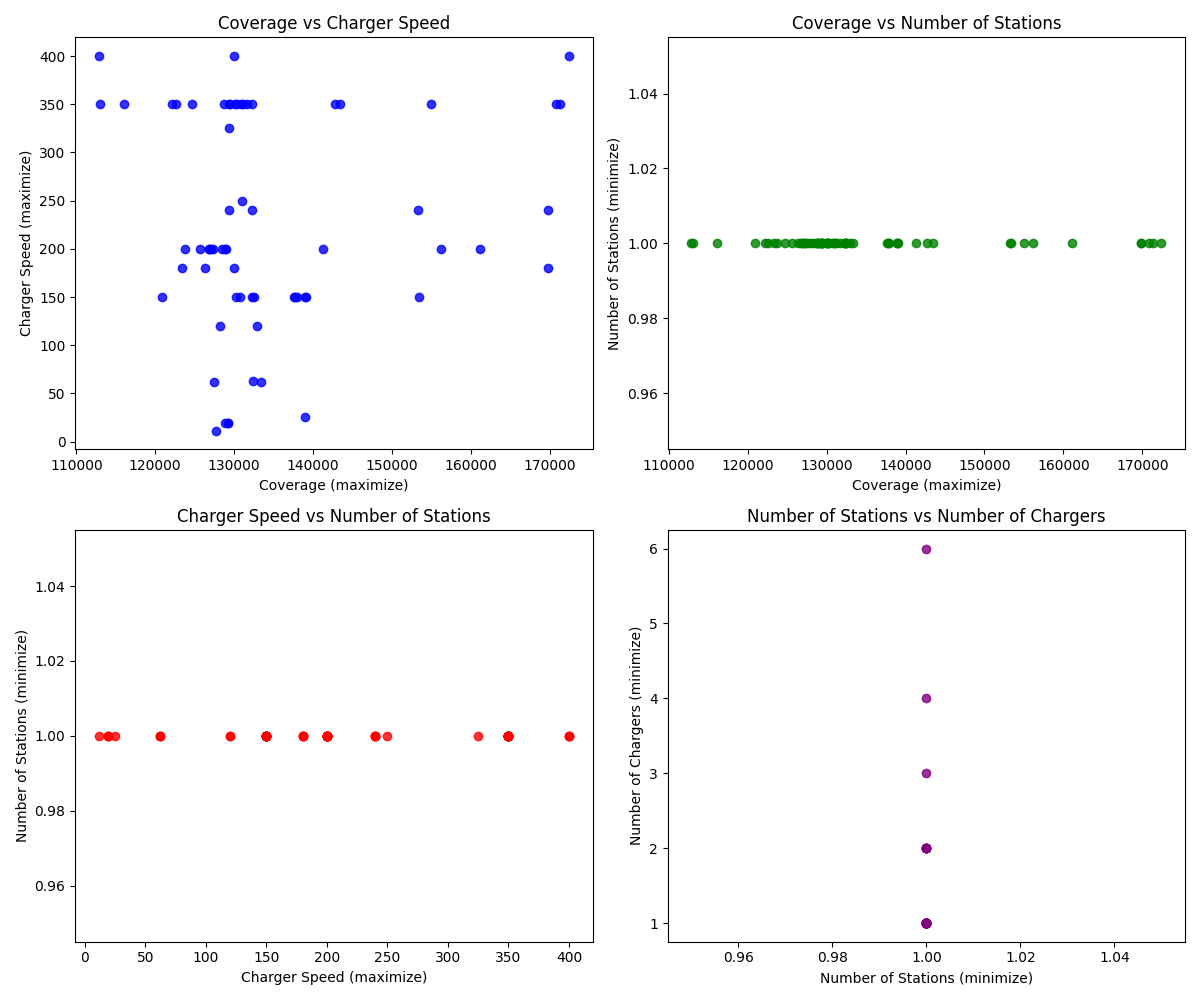
\includegraphics[width=0.7\textwidth]{../Figures/Trade_Off.png}
    \caption{Objective trade-offs among selected Pareto-optimal solutions.}
    \label{fig:trade_off}
\end{figure}

\subsection{Minimizing the Number of Stations and Chargers}
The optimization process achieved significant reductions in infrastructure, as shown in Figure~\ref{fig:Stations_Chargers}. The total number of EV charging stations (EVCS) decreased from 19 to 7, while the number of individual chargers dropped sharply from 69 to just 18. These reductions demonstrate the effectiveness of the algorithm in meeting the objective of minimizing infrastructure.

Reducing the number of stations and chargers leads to lower installation and maintenance costs, improved resource efficiency. This result highlights the practical benefits of using multi objective optimization to design streamlined and scalable EV charging station networks.


\begin{figure}[h!]
    \centering
    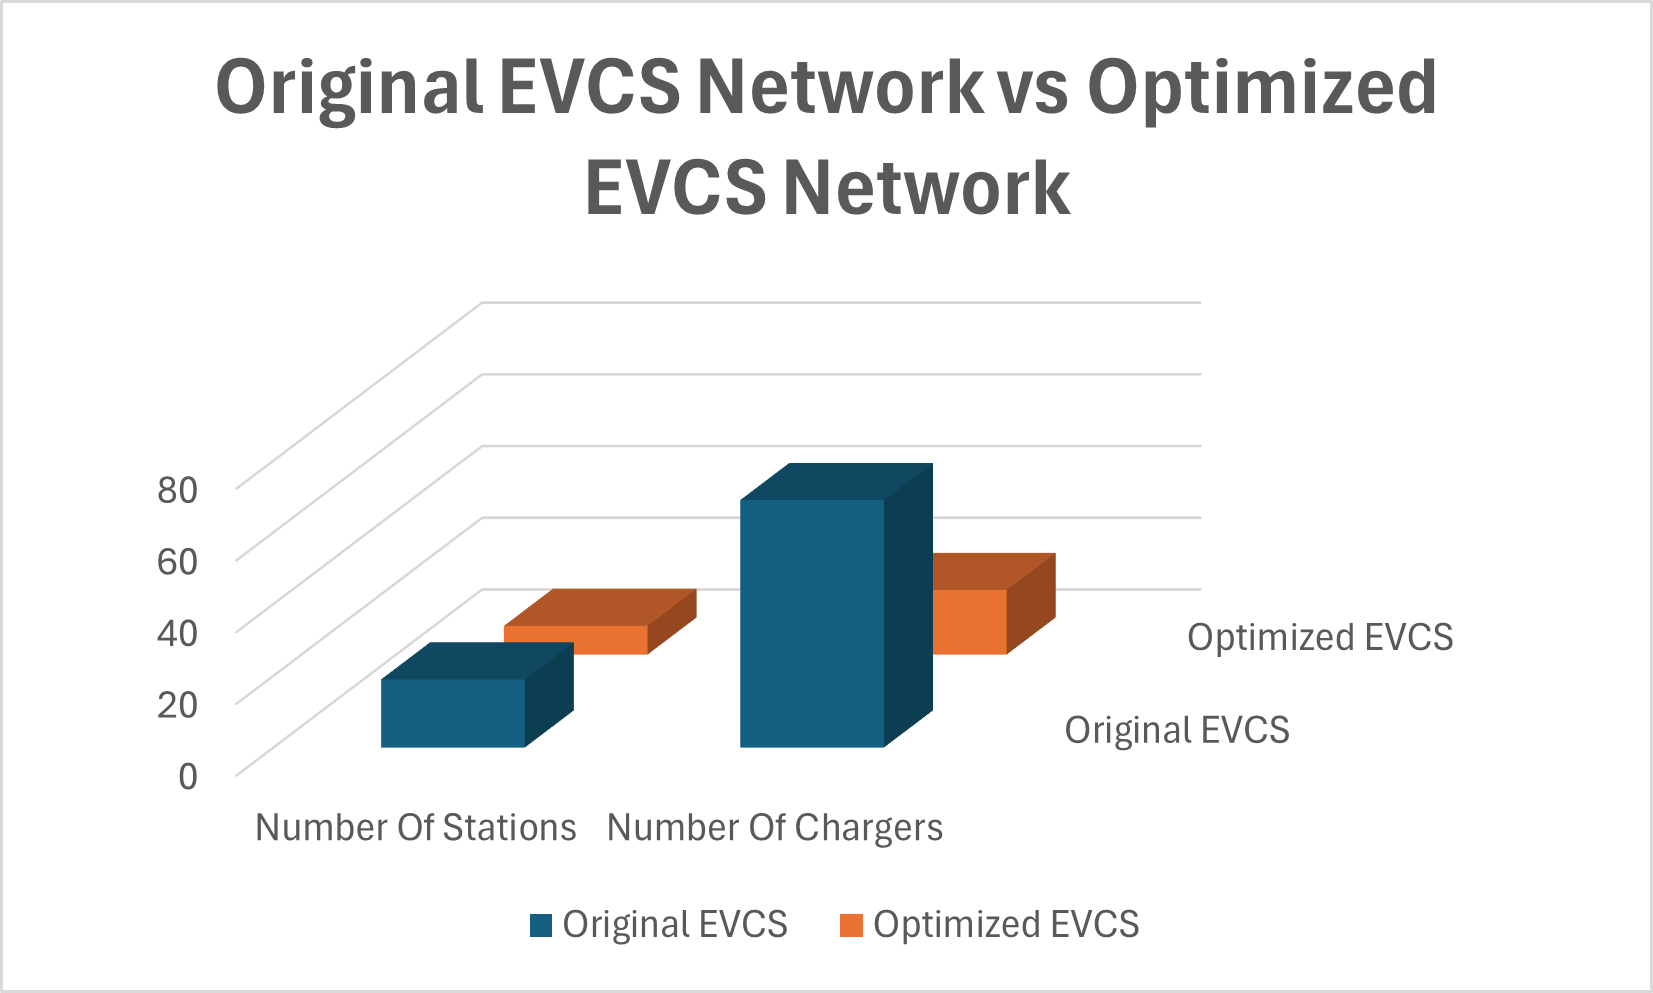
\includegraphics[width=0.7\textwidth]{../Figures/Original_vs_Optimized_evcs_network.png}
    \caption{Original EVCS Network vs Optimized EVCS Network.}
    \label{fig:Stations_Chargers}
\end{figure}

In addition, it's important to understand that these improvements were achieved through a multi-objective optimization process. Various objectives, such as maximizing coverage, increasing charger speed, and minimizing the average distance between EVs and the nearest charging station, must be carefully balanced.

Therefore, while the reduction in the number of stations and chargers is promising, it is the result of coordinating multiple competing objectives, rather than focusing solely on reducing infrastructure usage.

However, the reduction in infrastructure without severely compromising other objectives highlights the strength of the applied optimization approach. 

\subsection{Maximizing Charger Speed}

Enhancing charger speed was a key objective in improving the overall performance and user experience of the EVCS network. The optimization process prioritized upgrading chargers to Level 3, guaranteeing speeds of at least 50 kW. Charger power levels were then strategically adjusted based on local demand to optimize efficiency and service quality.

Figure~\ref{fig:Original_Chargers_Speed_vs_Optimized_Chargers_Speed}, and Figure~\ref{fig:Original_Chargers_Number_vs_Optimized_Chargers_Number}shows that many of the slower chargers were upgraded in the optimized data set to improve the overall network performance. Additionally, some high-power chargers were adjusted to better suit local demand.

In areas where very high charging power was unnecessary, these chargers were downgraded to lower capacities, such as 50 kW, to improve efficiency and reduce excess infrastructure.

\begin{figure}[h!]
\centering
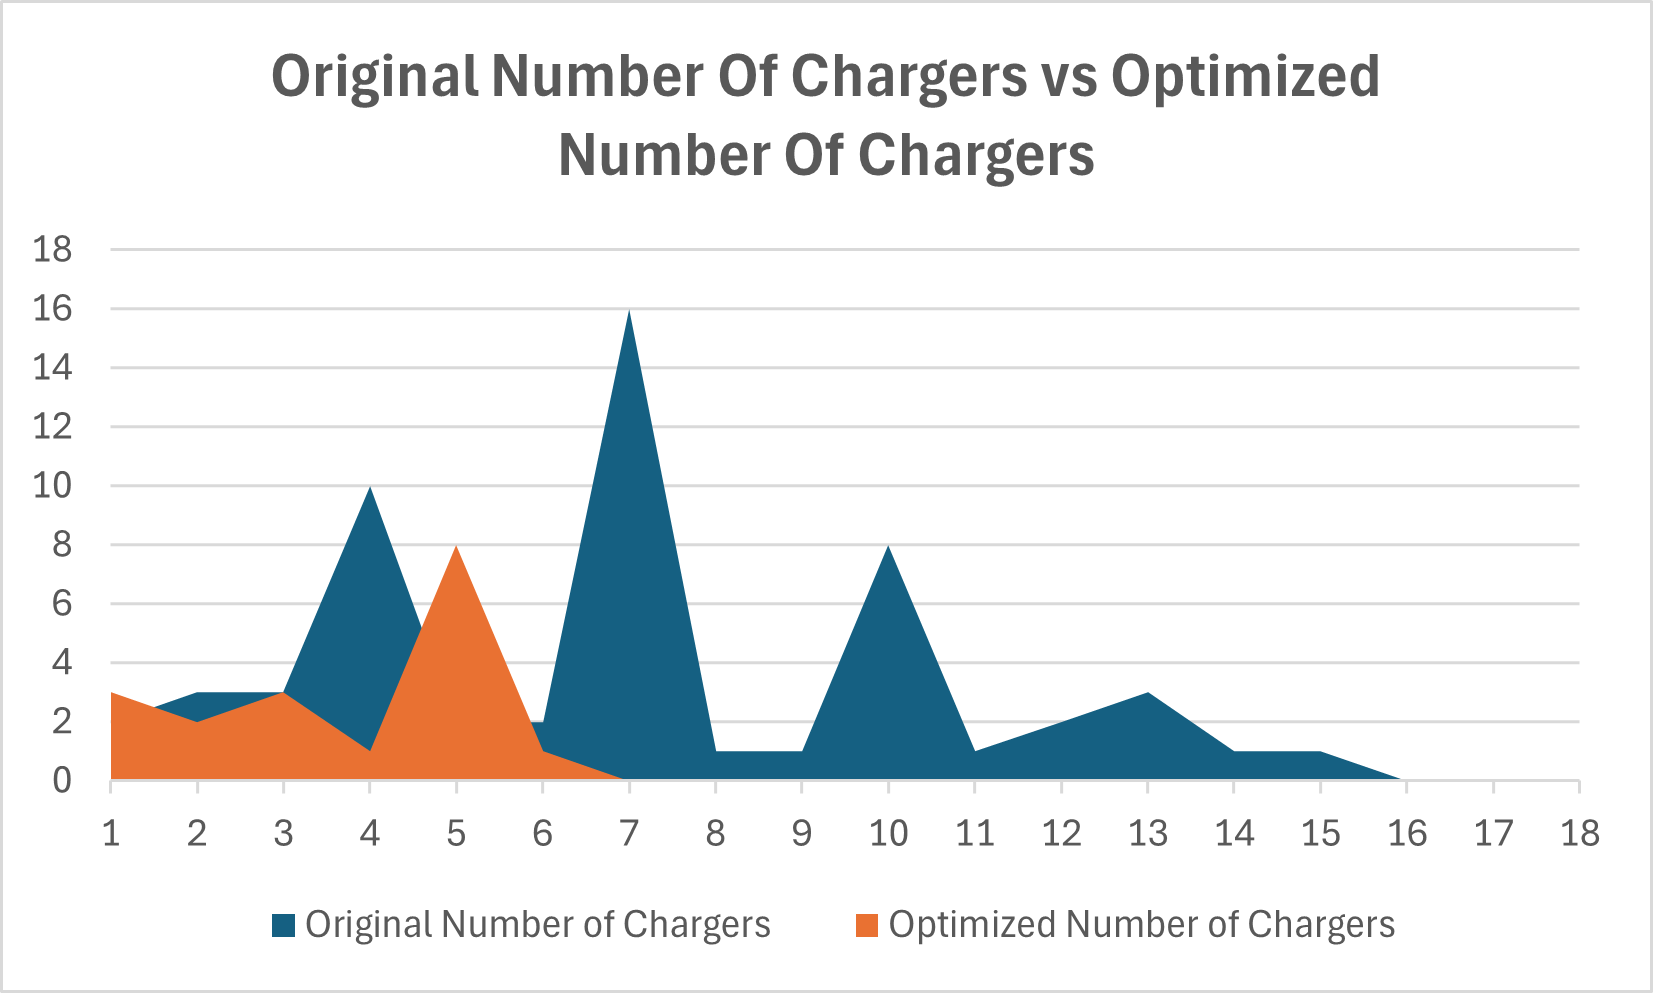
\includegraphics[width=0.7\textwidth]{../Figures/Original_vs_Optimized_evcs_chargers_number.png}
\caption{Comparison of original and optimized EVCS charger numbers.}
\label{fig:Original_Chargers_Number_vs_Optimized_Chargers_Number}
\end{figure}

\begin{figure}[h!]
\centering
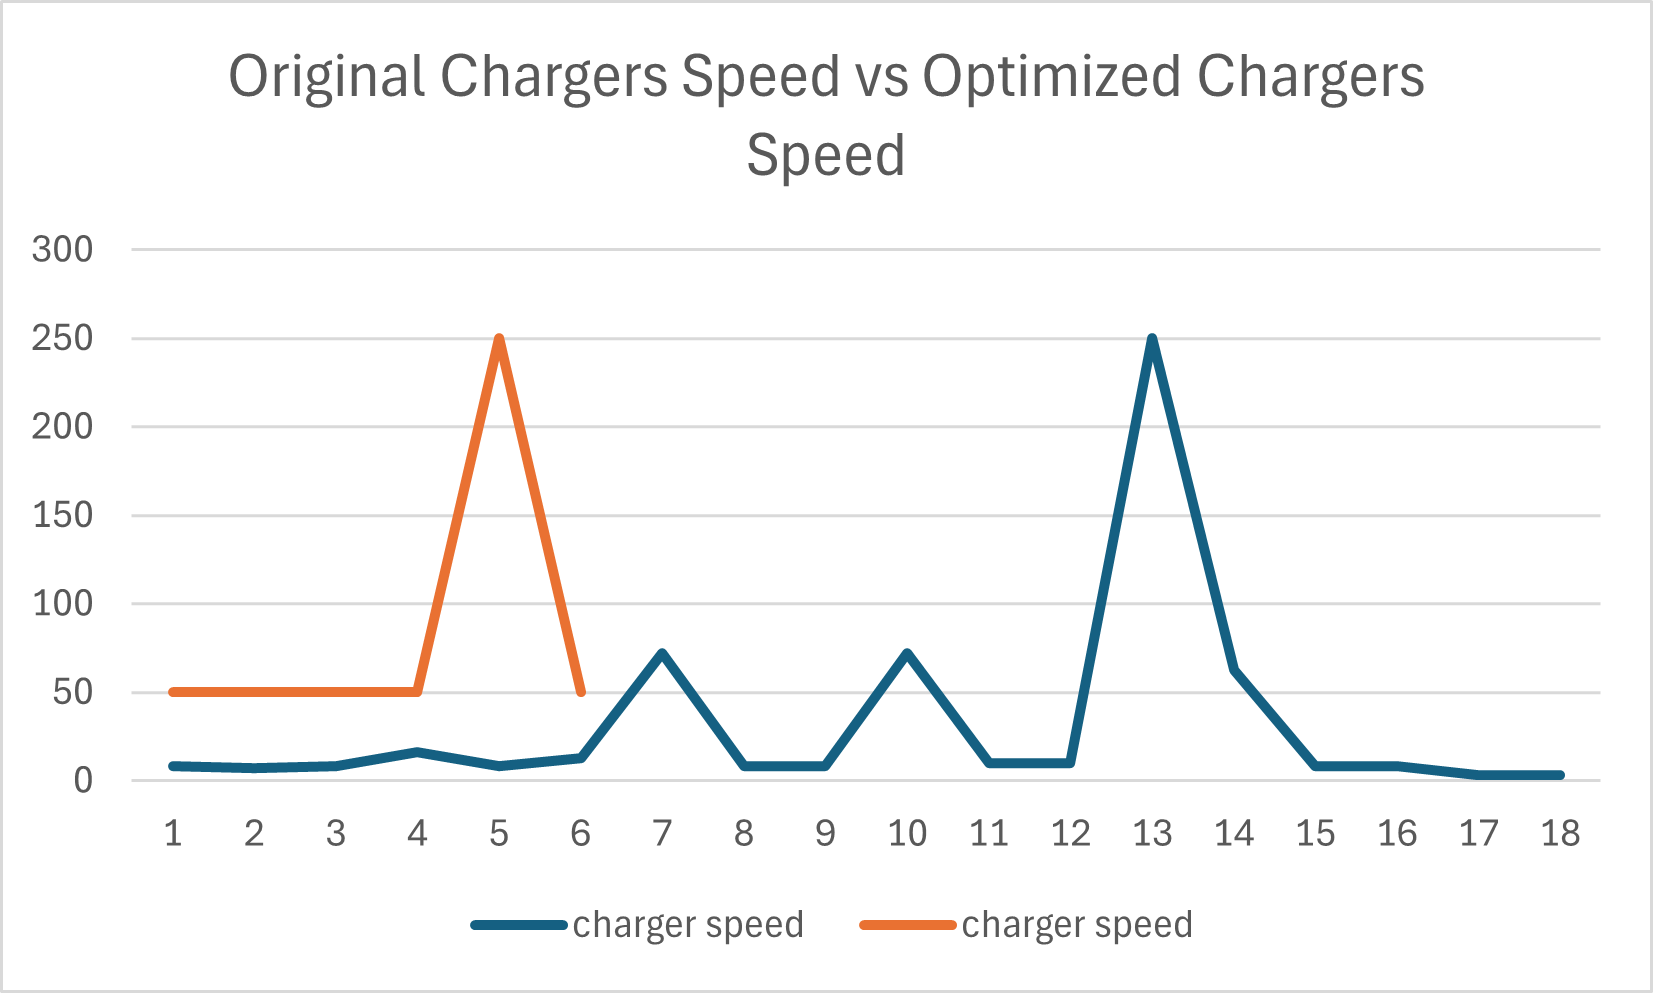
\includegraphics[width=0.7\textwidth]{../Figures/Original_vs_Optimized_evcs_chargers_speed.png}
\caption{Comparison of original and optimized EVCS charger speeds.}
\label{fig:Original_Chargers_Speed_vs_Optimized_Chargers_Speed}
\end{figure}

In addition, the reconfiguration of charger speeds shifts from a one-size-fits-all approach to a more tailored, data-driven strategy. By aligning charger capacities with local demand, the optimization process enhances system reliability while minimizing unnecessary costs. This balance is crucial for developing efficient, cost-effective, and scalable EV charging networks.


\subsection{Maximizing Coverage and Minimizing Average Distance}

The results for coverage did not fully meet expectations, and this is mainly due to the trade-offs involved in the multi-objective optimization process. Figure~\ref{fig:EVCS coverage} shows the first objective—maximizing coverage per station—which was expected to increase overall station coverage. However, since this study used a multi-objective approach, the algorithm had to balance several goals instead of focusing on just one. As a result, coverage per station didn’t improve as expected. This is especially clear when looking at Objective nummber (5), which focuses on minimizing the average distance between electric vehicles (EVs) and the nearest charging station, as shown in Figure 2. To reduce this distance, the algorithm made trade-offs, which meant that coverage at each station was somewhat limited. This highlights how multi-objective optimization involves balancing different goals, where improving one objective can impact another.

\begin{figure}[h!]
\centering
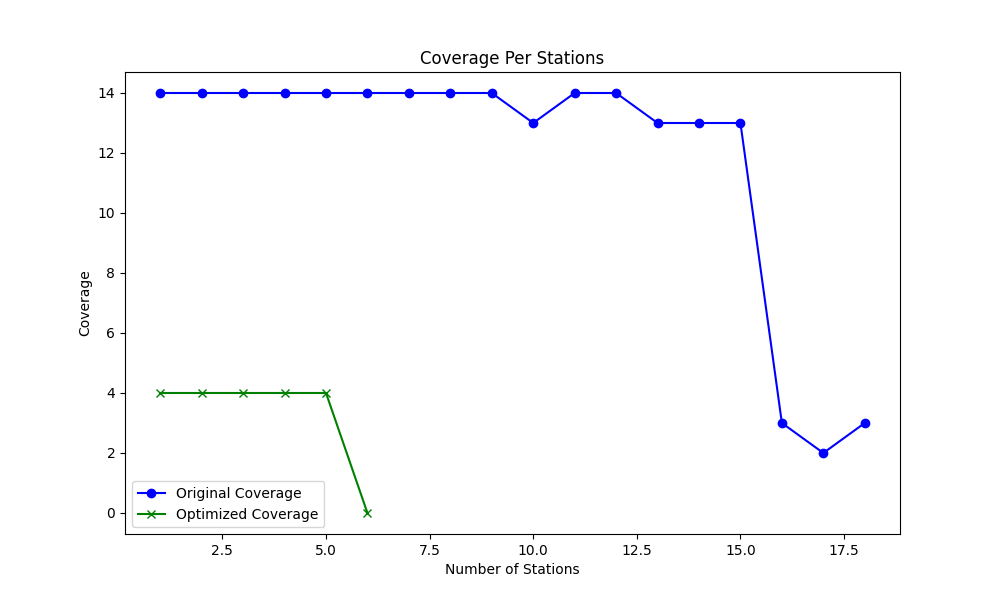
\includegraphics[width=0.7\textwidth]{../Figures/coverage_stations.png}
\caption{EVCS coverage per station.}
\label{fig:EVCS coverage}
\end{figure}

In addition, optimizing EVCS locations was an important outcome of the NSGA-II algorithm. Figures~\ref{fig:location_before} and~\ref{fig:location_after} compare the original EVCS network layout with the optimized configuration. The optimized layout shows a better distribution of stations, particularly in high-demand areas and along important transportation routes. This more strategic placement improves coverage overall and reduces the average distance between EVs and their nearest station, showing how the algorithm improves both service accessibility and infrastructure efficiency.

\begin{figure}[h!]
\centering
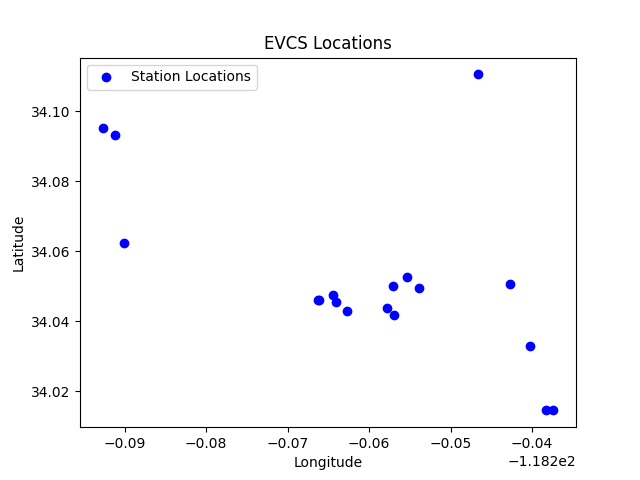
\includegraphics[width=0.7\textwidth]{../Figures/original_map.png}
\caption{EVCS locations before optimization.}
\label{fig:location_before}
\end{figure}

\begin{figure}[h!]
\centering
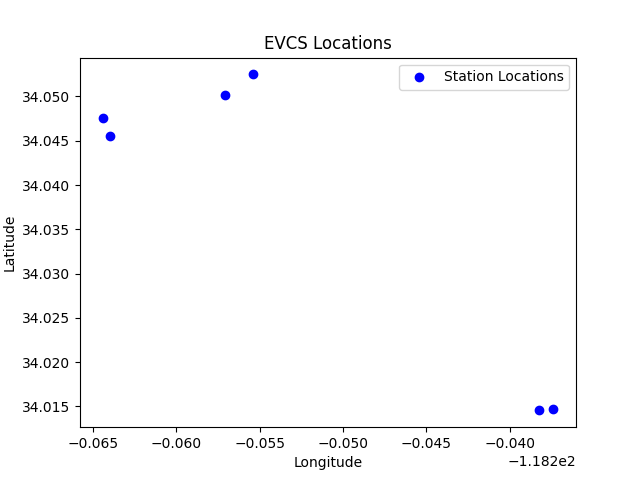
\includegraphics[width=0.7\textwidth]{../Figures/optimized_map.png}
\caption{EVCS locations after optimization.}
\label{fig:location_after}
\end{figure}

\newpage

As shown in Figure~\ref{fig:plot_distance}, the average distance between electric vehicles (EVs) and their nearest charging station is compared before and after the optimization process. The optimization results in a significant reduction in this distance, making the stations more accessible and convenient for users. The figure also shows the optimized EVCS layout, where fast chargers are placed in high demand areas, reducing travel distance while also effectively managing infrastructure costs.

\newpage

\begin{figure}[h!]
\centering
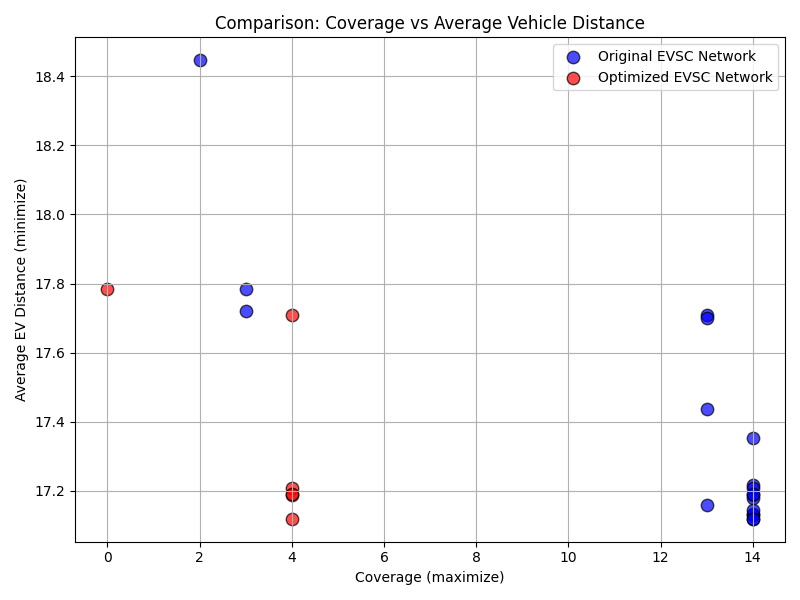
\includegraphics[width=0.8\textwidth]{../Figures/distance.png}
\caption{Average distance from EVs to their nearest EVCS before and after optimization.}
\label{fig:plot_distance}
\end{figure}
\newpage

This optimized configuration not only improves the efficiency of the EVCS network but also highlights the importance of considering both coverage and accessibility when designing charging infrastructure. By strategically placing chargers in high-demand areas and minimizing the distance to the nearest station, the optimization process ensures that the network is both cost-effective and user-friendly. These improvements will likely contribute to higher adoption rates of electric vehicles, as users can rely on a more accessible and convenient charging network. The success of this optimization approach demonstrates how data-driven methods can enhance the design of future EV charging systems to meet the growing demand for sustainable transportation.





\section{Minimizing Overall EVCS Infrastructure Costs}

To evaluate the impact of the optimization on the overall cost of electric vehicle charging infrastructure, Figure~\ref{fig:network_cost_comparison} presents a comparison of the network costs before and after the application of the NSGA-II algorithm. The results clearly show a substantial reduction in infrastructure expenditure in the optimized solution. This reduction was achieved by strategically minimizing the number of stations and chargers while maintaining the service coverage necessary for efficient EV charging. Importantly, the optimization ensures that the trade-off between cost reduction and accessibility is well-balanced, without compromising user convenience.

\clearpage

\begin{figure}[h!]
\centering
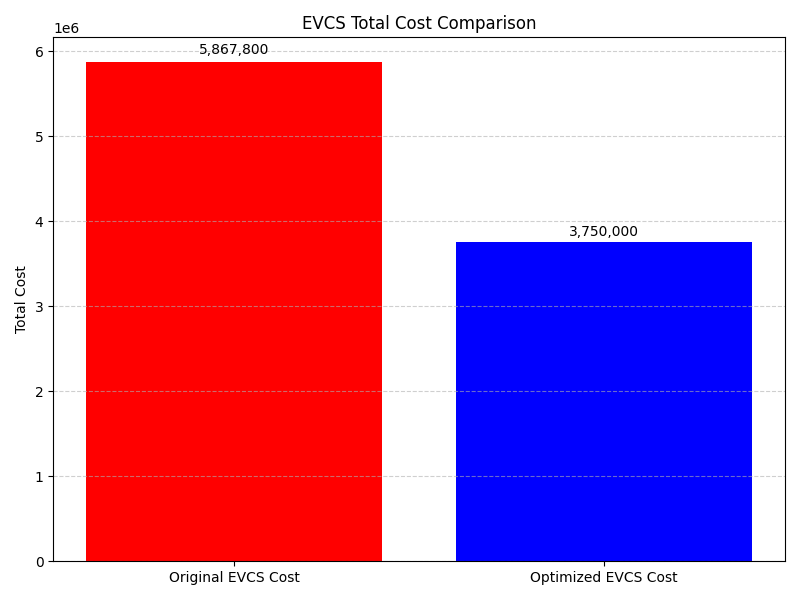
\includegraphics[width=0.7\textwidth]{../Figures/plot_EVCS_cost.png}
\caption{Network cost comparison before and after NSGA-II optimization.}
\label{fig:network_cost_comparison}
\end{figure}

The outcomes underscore the effectiveness of the NSGA-II algorithm in optimizing EV charging infrastructure across multiple objectives. By generating a diverse set of high-quality solutions, the algorithm allows for the exploration of various trade-offs between cost, coverage, and service efficiency. The results demonstrate not only a reduction in costs but also improvements in spatial coverage and a reduction in average travel distances for users. These improvements are critical for developing infrastructure that is both financially feasible and user-friendly. Further analysis of the results, presented through performance metrics in Section~\ref{sec:performance-metrics}, provides valuable insights for policymakers and urban planners. These findings can inform decisions aimed at deploying EVCS in a cost-effective, equitable, and scalable manner.


